\documentclass[12pt]{article}
\usepackage{preamble}

\pagestyle{fancy}
\fancyhead[LO,LE]{Теория вероятности}
\fancyhead[CO,CE]{24.09.2024}
\fancyhead[RO,RE]{Лекции Блаженова А. В.}

\fancyfoot[L]{\scriptsize исходники найдутся тут: \\ \url{https://github.com/pelmesh619/itmo_conspects} \Cat}

\begin{document}
    \subsection{Серия испытаний Бернулли}

    Схемой Бернулли - называется серия одинаковых независимых экспериментов, каждый из которых имеет 2 исхода: произошло интересующее нас событие или нет

    $p = p(A)$ - вероятность успеха при одном испытании

    $q = 1 - p$ - вероятность неудачи

    $v_n$ - число успехов в серии из $n$ испытаний

    $p(v_n = k) = p_n(k)$

    Из этого получаем формулу Бернулли:

    \begin{MyTheorem}
        \Ths Вероятность того, что при $n$ испытаниях произойдет ровно $k$ успехов, равна

        $p_n(k) = C_n^k p^k q^{n - k}$
    \end{MyTheorem}

    \begin{MyProof}
        $\Box$

        Рассмотрим один из элементарных исходов, благоприятных данному событию:

        $A_n = \underset{k}{\underbrace{\text{УУУ}\dots\text{У}}}\underset{n - k}{\underbrace{\text{Н}\dots\text{ННН}}}$ - $k$ успехов, $n - k$ неудачи

        $p(\text{У}) = p, p(\text{Н}) = q$

        Так как испытания независимы, то $p(A_n) = p^k q^{n - k}$

        Остальные элементарные исходы имеют ту же вероятность, перебираем все расстановки исходов, получаем $C_n^k$, в итоге, получаем формулу Бернулли

        $\Box$
    \end{MyProof}

    \Ex Вероятность попадания стрелка при одном выстреле - $0.8$. Какова вероятность того, что из пяти выстрелов точными будут три

    $n = 5 \quad p = 0.8 \quad q = 1 - p = 0.2 \quad k = 3$

    $p_5(3) = C^3_5 p^3 q^2 = 0.2048$

    \subsection{Наиболее вероятное число успехов}

    Выясним, при каком значении $k$ вероятность предшествующего числа успехов $k - 1$ будет не более, чем вероятность $k$ успехов

    $p_n(k - 1) \leq p_n(k)$

    $C_n^{k - 1} p^{k - 1} q^{n - k + 1} \leq C^k_n p^k q^{n - k}$

    $\frac{n!}{(k - 1)! (n - k + 1)!} q \leq \frac{n!}{(k)! (n - k)!} p$

    $\frac{q}{(k - 1)! (n - k + 1)!} \leq \frac{p}{(k)! (n - k)!}$

    $\frac{q}{n - k + 1} \leq \frac{p}{k}$

    $k(1 - p) \leq p(n - k + 1)$

    $k \leq np + p$

    Отсюда $np + p - 1 \leq k \leq  np + p$

    Рассмотрим 3 ситуации:

    1) $np$ - целое, тогда $np + p$ - нецелое, и $k = np$ - наиболее вероятное

    2) $np + p$ - нецелое, тогда $k = \lfloor np + p \rfloor$

    3) $np + p$ - целое, тогда $np + p - 1$ - целое, и 2 наиболее вероятных числа успеха

    Геометрическая интерпретация:

    \begin{center}
        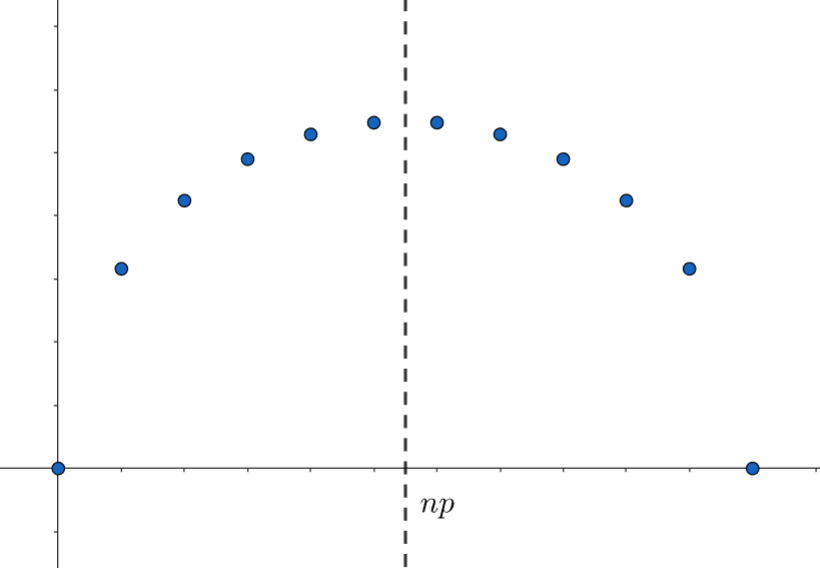
\includegraphics[width=6cm]{probtheory/images/probtheory_2024_09_24_1}
    \end{center}

    При увеличении числа $n$ точки превращаются в кривую Гаусса

    \begin{center}
        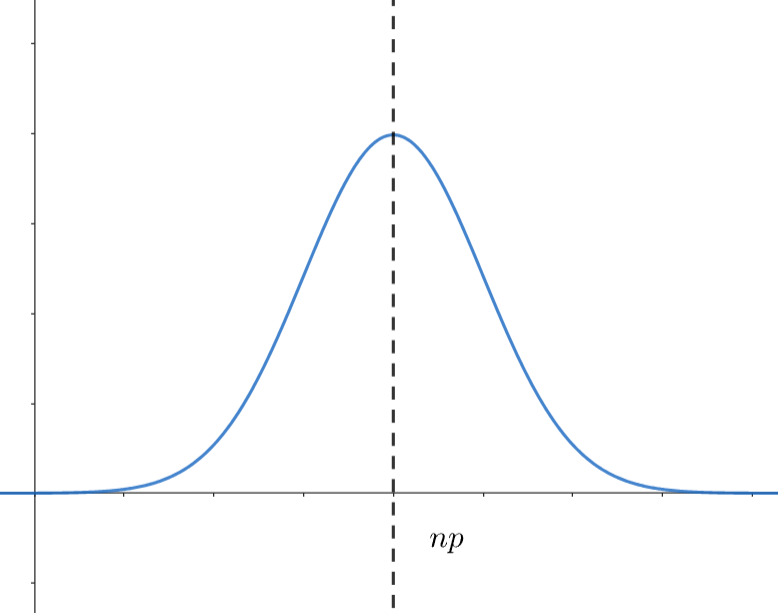
\includegraphics[width=6cm]{probtheory/images/probtheory_2024_09_24_2}
    \end{center}

    При увеличении числа испытаний $n$ формула Бернулли вырождается в следующие асимптотические формы (применяем, если требуется найти вероятность точного числа успеха)

    1) локальная формула Муавра-Лапласа

    $p_n(k) \underset{n \to \infty}{\longrightarrow} \frac{1}{\sqrt{npq}} \varphi(x)$, где $\varphi(x) = \frac{1}{\sqrt{2\pi}} e^{-\frac{x^2}{2}}$ - функция гаусса

    $x = \frac{k - np}{\sqrt{npq}}$

    Свойства $\varphi(x)$:

    1. $\varphi(x) = \varphi(-x)$ - функция четная

    2. при $x > 5 \quad \varphi(x) \approx 0$

    2) Интегральная формула Муавра-Лапласа (если требуется найти вероятность того, что число успехов в данном диапазоне)

    $p_n(k_1 \leq k \leq k_2) \underset{n \to \infty}{\longrightarrow} \Phi(x_2) - \Phi(x_1)$, где $\Phi(x) = \frac{1}{\sqrt{2\pi}} \int_0^x e^{-\frac{z^2}{2}} dz$ - функция Лапласа

    $x_1 = \frac{k_1 - np}{\sqrt{npq}}$ - отклонение от левой границы, $x_2 = \frac{k_2 - np}{\sqrt{npq}}$ - отклонение от правой

    Свойства $\Phi(x)$

    1. $\Phi(-x) = -\Phi(x)$ - функция нечетная

    2. при $x > 5 \quad \Phi(x) \approx 0.5$

    \Nota Эти формулы обычно можно применять при $n \geq 100$ и $0.1 \leq p \leq 0.9$

    \Nota В некоторых источниках под функцией Лапласа подразумевают другую функцию: $F_0(x) = \frac{1}{\sqrt{2\pi}} \int_{-\infty}^x e^{-\frac{t^2}{2}}dt$ - стандартное отклонение. Эта функция
    отличается от $F_0 = \frac{1}{\sqrt{2\pi}} \int_{-\infty}^0 e^{-\frac{t^2}{2}}dt + \Phi(x) = \frac{1}{2} + \Phi(x)$

    Так как $\int_{-\infty}^{\infty} e^{-x^2} dx = \sqrt{\pi}$ - интеграл Пуасона

    \Ex Вероятность попадания стрелка в цель $0.8$, стрелок сделал 400 выстрелов. Найти вероятность того, что:

    а) произошло ровно 330 попаданий

    б) произошло от 312 до 336 попаданий

    а) $x = \frac{k - np}{\sqrt{npq}} = \frac{330 - 400 \cdot 0.8}{\sqrt{400 \cdot 0.8 \cdot 0.2}} = \frac{330 - 320}{8} = 1.25$

    $p_{400}(330) \approx \frac{1}{\sqrt{npq}} \varphi(1.25) = \frac{1}{8} \varphi(1.25) \approx \frac{1}{8} \cdot 0.1826 \approx 0.0228$

    б) $x_1 = \frac{312 - 320}{8} = -1$, $x_2 = \frac{336 - 320}{8} = 2$

    $p_{400}(312 \leq k \leq 336) \approx \Phi(2) - \Phi(-1) = \Phi(2) + \Phi(1) \approx 0.4772 + 0.3413 = 0.8185$

    \subsection{Статистическое понятие вероятности}

    Пусть проводим $n$ реальных экспериментов, $n_A$ - число появления события $A$, $\frac{n_A}{n}$ - относительная частота события $A$.

    Эксперименты с монетой показали, что при больших $n$, $\frac{n_A}{n} \approx p(A)$ - явление стабилизации

    Вероятность отклонения относительной частоты от вероятности события

    $n$ - число испытаний, $p = p(A), \frac{n_A}{n}$ - экспериментальная частота

    $p\left(|\frac{n_A}{n} - p| \leq \varepsilon\right) = p\left(-\varepsilon \leq \frac{n_A}{n} - p \leq \varepsilon\right) = p(-n\varepsilon \leq n_A - np \leq n\varepsilon) = p(np - n\varepsilon \leq n_A \leq n\varepsilon + np) \underset{n \to \infty}{\longrightarrow}$ [по интегральной формуле Лапласа] $\underset{n \to \infty}{\longrightarrow} \Phi\left(\frac{n\varepsilon}{\sqrt{npq}}\right) - \Phi\left(-\frac{n\varepsilon}{\sqrt{npq}}\right)$

    $ = \Phi\left(\frac{\sqrt{n}\varepsilon}{\sqrt{pq}}\right) - \Phi\left(-\frac{\sqrt{n}\varepsilon}{\sqrt{pq}}\right)$

    $ = 2\Phi\left(\frac{\sqrt{n}\varepsilon}{\sqrt{pq}}\right)$

    Итак, получили, что нужная нам вероятность $p\left(|\frac{n_A}{n} - p| \leq \varepsilon\right) \approx 2\Phi\left(\frac{\sqrt{n}\varepsilon}{\sqrt{pq}}\right)$

    \subsection{Закон больших чисел Бернулли}

    Итак, $p\left(|\frac{n_A}{n} - p| \leq \varepsilon\right) \underset{n \to \infty}{\longrightarrow} 2 \Phi\left(\frac{\varepsilon}{\sqrt{pq}}\sqrt{n}\right)$

    при $n \to \infty, \sqrt{n} \to \infty, \frac{\varepsilon}{\sqrt{pq}} \sqrt{n} \to \infty, \Phi\left(\frac{\varepsilon}{\sqrt{pq}}\sqrt{n}\right) \to 0.5, p\left(|\frac{n_A}{n} - p| \leq \varepsilon\right) \to 2 \cdot 0.5 = 1$ - закон больших чисел показывает, что вероятность попадания относительной частоты в $\varepsilon$-трубу вероятность события приближается к 1

    $\lim_{n \to \infty} p\left(|\frac{n_A}{n} - p| \leq \varepsilon\right) = 1$ или $\frac{n_A}{n} \underset{n \to \infty}{\longrightarrow} p$ - сходимость по вероятности

    \Ex Для оценки доли $p$ курящих людей берется выборка объема $n$, и делается оценка доли курящих людей по формуле $p^* = \frac{n_A}{n}$.
    Каким должен быть объем $n$, чтобы с вероятностью $\gamma = 0.95$ данная оценка отличалась от истинного значения не более, чем на $\varepsilon = 0.01$

    По формуле вероятности отклонения частоты от вероятности $p(|p^* - p| \leq \varepsilon) = p\left(|\frac{n_A}{n} - p| \leq \varepsilon\right) \approx 2\Phi\left(\frac{\varepsilon}{\sqrt{pq}}\sqrt{n}\right) = 0.95$

    $\Phi\left(\frac{\varepsilon}{\sqrt{pq}}\sqrt{n}\right) = 0.475$

    $\frac{\varepsilon}{\sqrt{pq}}\sqrt{n} = 1.96$

    $\frac{1}{\sqrt{pq}}\sqrt{n} = 196$

    $\frac{n}{pq} = 38416$

    $n \geq 38416 pq$

    В самое худшей ситуации $pq \leq 0.5^2 = \frac{1}{4}$

    $n \geq \frac{38416}{4} = 9604$


\end{document}
